\chapter{System Architecture}
In this chapter, we propose a design for our system. We will use the
principles that we laid down in the previous chapter and present them
as a part of an integrated system

\section{General concepts and overall goal}
With security as the, as previously stated, principal goal, we focus
our design around several small processes, each with a well defined
purpose and interactions. We furthermore enforce a principle of
minimum permissions across our entire system. This means that we eill 

\section{Users}
There are two levels of users in the OnlineTA system. One is the user
owning the daemons responsible for handling the main assessment flow,
and the other is the users owning the submissions. In the case of
anonymous submissions 

\subsection{Representing systems on users}
Name lookup services in GNU/Linux systems are handled by the NSS (Name
Service Switch) subsystem which is implemented in the Gnu glibc library. The NSS
service is responsible for handling the mapping of several system
resources including domain names, user names and password files. The
NSS system is extensible through providers which is called in the
order specified by the \texttt{nssswitch.conf} file. In the OnlineTA
system, we add a password mapping module which can be used for looking
up user names to UIDs and vice-verca\cite{nss}.

This allows us to represent our dynamically created users on the Linux
system and thus avoid having to fill all of them into an extremely
long /etc/passwd file.

We perform user handling in two separate NSS modules for handling
named an anonymous submission respectively. The usernames of
identified submissions are assigned by a NSS module which implements
the bidirectional UID to KU-username mapping previously described.
conversion scheme previously described.

We handle the usernames of anonymous submissions slightly
differently through a different NSS module. This module works on lists
of preallocated users and is autonomously responsible for maintaining
lists of allocated and non-allocated users \fxnote{rewrite}


\section{Interactions}
The scope of the current implementation is limited to supporting
direct interactions via a web browser, however, the additional modes
of interaction previously described can be implemented on top of the
interface that we will describe in this section.

In the current design, all interactions with the system occurs over a
secure HTTP connection. We use the first part of the request URI to
determine which action is requested by the user while subsequent URI
components are used as parameters for that request. The system
supports the following actions:

\begin{description}

\item[\texttt{/}] This URI can be issued as a HTTP GET request and
  will return the main index page which will contain a list of courses
  and assignments availiable on that server
\item[\texttt{/submit/<course>/<assignment>/}] When a HTTP POST
    request is issued to this URL it will be handled as an anonymous
    submission. If the submission is accepted, the fronted will
    repsond with a page showing the assigned submission UUID. This
    UUID can then be used in order to retrieve assessments once they
    are completed
\item[\texttt{/submit/<course>/<assignment>/<KU-username>}] This
  request type is the same as the previous except that it will perform
  an authenticated submission.
\item[\texttt{/query/<uuid>}] Used to query assessment status of
  assignment identified by given UUID. The status of an assignment can
  be the following ACCEPTED The assignment has been accepted and is
  awaiting schediling QUEUED The assignment has been picked up by the
  scheduler and is awaiting prioirization TODO
\item[\texttt{/assessment/<uuid>}] Retrieves the assessment of a
  submission if availible
\end{description}

\subsection{Relaying assessment to user}
TODO: Describe what happens when a user requests an assessment.

\section{Components}
The components that our design is separated into are the following:

\begin{figure}
\centering
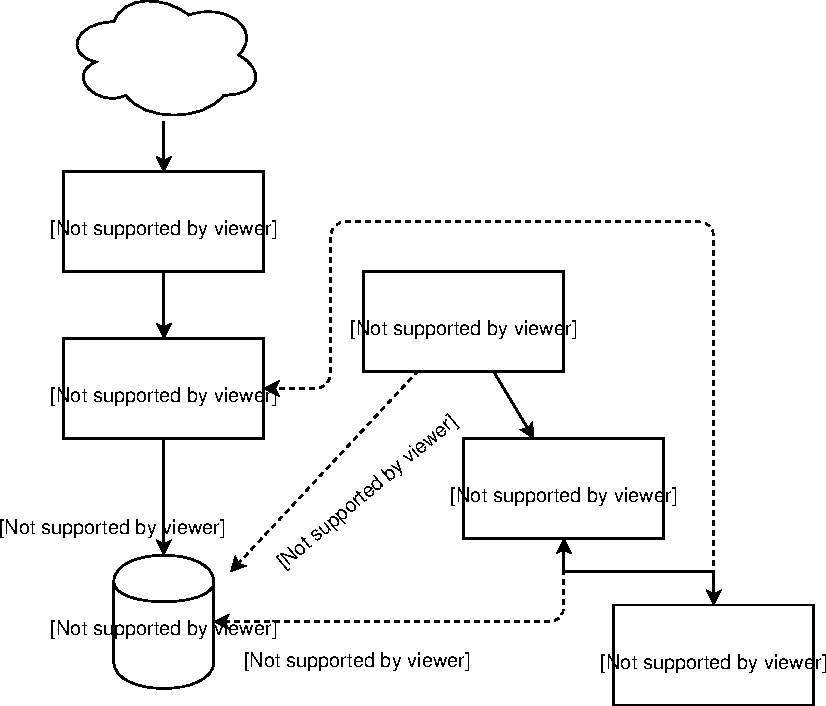
\includegraphics[width=\textwidth]{figures/arch}
\caption{Flowchart showing interactions between the components of the
  OnlineTA system}
\label{fig:arch}
\end{figure}

\paragraph{Frontend}
The frontend is responsible for accepting submissions. In case of
authenticated submissions it is also responsible for verifying the
identity of the user submitting the assignment. It will also perform
the initial storage of the submission. Furthermore, the frontend is
responsible for returning the assessment to the student.

It will go through the following steps in order to accept an
assignment.

The frontend has the following roles
\begin{itemize}
\item Accepting submissions from the HTTP proxy
\item Verify GPG signature of submission if authenticated
\item Generating and assigning a UUID to the submission
\item Writing the initial metadata file
\item Creating directory for containing the submission and setting
  ownership of files
\end{itemize}

This component require the \texttt{CAP\_CHOWN} capability.

\paragraph{Scheduler}
The scheduler will pick up the assignment after it has been saved to
disk and pair it with a suitable assessment unit. Assignment
scheduling is based primarily on a priority assigned to the submission
by the frontend. Submissions with equal priorities are scheduled on a
FIFO basis. If no priority is provided by the assignment, it could
assign a priority based on a number of factors, e.g. time remaining
before submission deadline. The scheduler directly spawns processes for
executing assessment units.

The scheduler has the following roles:
\begin{itemize}
\item Monitoring the incoming directory for new submissions
\item Pairing submissions with an appropriate assessment unit
\item Scheduling and prioritizing assessment of assignments
\item Invoking workers for performing the actual assignment
\end{itemize}

\paragraph{Worker}
A worker process is spawned by the scheduler and its overall purpose
is to set up and initiate the assessment process. It is initially
started as the \texttt{onlineta} user but after the assessment
environment has been configured and the containers has been created it
will \texttt{suid} to the user owning the submission and shed its special
capabilities.

Specifically, its roles are the following
\begin{itemize}
\item Setting up the environment for performing an assessment
  including mounting filesystems
\item Setting up containers for assessment
\item Relaying assessment to frontend
\end{itemize}

The special capabilities required by the Worker process are
\texttt{CAP\_SYSADM}, \texttt{CAP\_SUID} and \texttt{CAP\_SETPCAP}

\paragraph{Assessment units}
An assessment unit handles the actual assessment of an assignment... TODO

\section{Storage}
In our current design, availability of persistent local disk storage
is assumed. The directory structure used for storing submission data
is as follows:

\begin{description}
\item{\texttt{submissions}} The parent of the directory tree
\item{\texttt{<UUID>}} A directory named after the UUID assigned to
  a submission is placed as a sub directory of the submissions
  directory. It holds all the files related to a submission, including
  it's assessment.  he contents of this directory are owned by the user
  who made the submission and thus it can only be accessed by an
  assessment unit running as this user.
\item{\texttt{incoming}} This directory is where the metadata files of
  all newly created directories are stored. It is monitored by the
  scheduler using \texttt{inotify} which, after a metadata file is
  scheduled it is moved away from this directory
\item{\texttt{accepted}} This directory holds metadata files which has
  been accepted for processing. The separation of incoming and
  accepted metadata files is needed due to limitations of inotify \fxnote{elaborate}
\end{description}

\fxnote{Make actual figure}
\begin{verbatim}
    submissions
       /|\
      / | \
     /  |  +-----+---------+
    /   |        |         |
UUID1   UUID2   UUID3   metadata
                           /\
      --------------------+  \
     |                   /    \
     |        UUID1.metadata UUID2.metadata
  incoming
     |
   UUID3.metadata

\end{verbatim}


\section{Interfaces}


\section{Scaling and distributing}
A driving idea behind our design is to enable horizontal
scalability. A key element to acheiving this


%%% Local Variables:
%%% mode: latex
%%% TeX-master: "master"
%%% TeX-command-extra-options: "-enable-write18"
%%% End:
